%
% File emnlp2020.tex
%
%% Based on the style files for ACL 2020, which were
%% Based on the style files for ACL 2018, NAACL 2018/19, which were
%% Based on the style files for ACL-2015, with some improvements
%%  taken from the NAACL-2016 style
%% Based on the style files for ACL-2014, which were, in turn,
%% based on ACL-2013, ACL-2012, ACL-2011, ACL-2010, ACL-IJCNLP-2009,
%% EACL-2009, IJCNLP-2008...
%% Based on the style files for EACL 2006 by 
%%e.agirre@ehu.es or Sergi.Balari@uab.es
%% and that of ACL 08 by Joakim Nivre and Noah Smith

\documentclass[11pt,a4paper]{article}
\usepackage[hyperref]{emnlp2020}
\usepackage{times}
\usepackage{latexsym}
\renewcommand{\UrlFont}{\ttfamily\small}

% This is not strictly necessary, and may be commented out,
% but it will improve the layout of the manuscript,
% and will typically save some space.
\usepackage{microtype}

\usepackage{times}
\renewcommand*\ttdefault{txtt}
\usepackage{soul}
\usepackage{url}
%\usepackage[hidelinks]{hyperref}
%\usepackage[utf8]{inputenc}
%\usepackage[small]{caption}
\usepackage{graphicx}
\usepackage{amsmath}
\usepackage{booktabs}
\urlstyle{same}

\usepackage{footnote}
\usepackage{array}
\usepackage{soul}
\usepackage{color}
\usepackage[utf8]{inputenc}
\usepackage{amsmath}
\usepackage{multirow}
%\usepackage{algorithm}
%\usepackage{algorithmicx}
%\usepackage{algpseudocode}
\usepackage[linesnumbered,boxed,ruled,commentsnumbered]{algorithm2e}
\newcommand{\figref}[1]{Figure \ref{#1}}
\newcommand{\eqnref}[1]{Eq. \ref{#1}}
\newcommand{\tabref}[1]{Table \ref{#1}}
\newcommand{\secref}[1]{Section \ref{#1}}
\newcommand{\algoref}[1]{Algorithm \ref{#1}}

\aclfinalcopy % Uncomment this line for the final submission
\def\aclpaperid{215} %  Enter the acl Paper ID here

\setlength\titlebox{6cm}
% You can expand the titlebox if you need extra space
% to show all the authors. Please do not make the titlebox
% smaller than 5cm (the original size); we will check this
% in the camera-ready version and ask you to change it back.

\newcommand\BibTeX{B\textsc{ib}\TeX}

\title{Multi-turn Response Selection using Dialogue Dependency Relations}

\author{Qi Jia$^1$ \hspace*{1cm}
	Yizhu Liu$^2$ \hspace*{1cm}
  	Siyu Ren$^3$ \hspace*{1cm} Kenny Q. Zhu$^4$\thanks{\hspace{2mm}The corresponding author.}\\
  Shanghai Jiao Tong University \\
  Shanghai, China \\
  \texttt{\{$^1$Jia\_qi,$^2$liuyizhu,$^3$roy0702\}@sjtu.edu.cn} \hfill
  \texttt{$^4$kzhu@cs.sjtu.edu.cn} \\ 
  \AND
%  Kenny Q. Zhu \\
%  Shanghai Jiao Tong University \\
%  Shanghai, China \\
%  \texttt{kzhu@cs.sjtu.edu.cn} \\\And
  Haifeng Tang \\
 China Merchants Bank Credit Card Center\\
  Shanghai, China \\
  %Affiliation / Address line 3 \\
  \texttt{thfeng@cmbchina.com} \\
}

\date{}	

\begin{document}
\maketitle
\begin{abstract}
Multi-turn response selection is a task designed for developing dialogue agents. The performance on this task has a remarkable improvement with
pre-trained language models. However, these models simply concatenate the turns in dialogue history as the input and largely ignore the dependencies between the turns. In this paper,  we propose a dialogue extraction algorithm to transform a dialogue history into threads based on their dependency relations. Each thread can be regarded as a self-contained sub-dialogue. We also propose Thread-Encoder model to encode threads and candidates into compact
representations by pre-trained Transformers and finally get the matching score through an attention layer. The experiments show that dependency relations are helpful for dialogue context understanding, and our model outperforms the state-of-the-art baselines on both DSTC7 and DSTC8*, with competitive results on UbuntuV2.
\end{abstract}
\section{Introduction}

Protein$-$protein interactions (PPIs) are of central importance for the majority of biological functions, such as signal transduction, metabolic pathways, molecular dynamics, and protein networks\cite{Hoffmann.Krallinger.ea:2005}, for they serve as the most fundamental building blocks of the entire interacademic systems of any organisms. Collecting data on pairwise interaction relationships is essential for multiple purpose, including identification of modules with certain functionality\cite{Spirin.Mirny.03}, mapping diseases to dominated genes\cite{Ideker.Sharan.08}, and after all, understanding wholistic metabolic/genetic networks from a system biology perspective.

A lot of databases have been built to store protein and genetic interactions from major model organism species and are available in various standardized formats, such as MINT\cite{Zanzoni.Montecchi-Palazzi.ea:2002}, BIND\cite{Bader.ea:2003}, BIOGRID\cite{DBLP:journals/nar/StarkBRBBT06}, etc. Among those mainstream databases, the data largely rely on voluntary reports by scientists or researchers, besides, comprehensive curation efforts become indispensable for the sake of accuracy. However, the amount of biology-related literatures with respect to protein interactions grows explosively and thus make it either impossible or impractical to manually detect PPI information anymore.

Considering huge amount of PPI information with great wealth hidden in published papers, in recent years, numerous mining techniques have been proposed that aim to extract PPI information automatically from free text, especially machine learning, information retrieval, and natural language processing\cite{DBLP:journals/bib/WinnenburgWPDS08}.These approaches can be roughly categorized into three classes: co$-$occurrence, rule$-$based, and machine learning. 

Co$-$occurrence is the approach with most simplicity and naivete. Just as its name implies, this method intends to find out pairs of proteins that co-occur in the same context. The scope of "same context" ranges from phrase, sentence, paragraph to whole abstract, even document. The underlying assumption is that whenever two proteins are mentioned together by authors, chances are high that there is some kind of relationship between them. However, however, in-context closeness even semantic relation does not necessarily represent actual biological interaction. As a consequence, a large fraction of candidate pairs are mismatched inevitably, causing a high recall but low precision.

The second approach is rule-based extraction, in other words, pattern matching. There are many types of rules, most of them concern natural language processing (NLP). One way is to specify hand-crafted regular expressions before hand, which mostly lean on language usage preference. Besides, by using full or partial (shallow) parsing strategies, more information would be acquired, such as part-of-speech taggers, local dependencies between syntactic components, context-free grammar\cite{DBLP:journals/bioinformatics/TemkinG03}, and full sentence structure. Compared to co$-$occurrence, rule-based approach enjoy better precision but much lower recall. In addition, since the rules are usually derived from training data, that is to say, the improper choice of training data would be significantly lethal, therefore quality of extraction is invariably instable and may not applicable to other data.

The third and most commonly used approach use machine learning techniques, in this case, the task to extract protein$-$protein interactions turns out to be a binary classification problem. Each protein pairs are represented along with a set of features, which is associated with their context, then a well$-$defined classifier gives the answer whether the candidate protein pairs is classified to be qualified PPI. (TO BE FURTHER FILLED!!!)

In this paper, we introduce a general bootstrapping framework for Protein$-$protein interaction extraction from natural text.Our method differs from most of the previous works in three aspects:

(1)The extraction process is driven by only tiny fraction of training data, which are regarded as seed data. In each round, it would derive reliable patterns automatically from seed data, then extract more positive PPI pairs consequently, what's more, the seed data would be augmented by the newly extracted results with high confidence.

(2)multiple graph kernel. 

(3)various evaluation.









\section{Approach}
%We first present our methods for testing short circuits in
%models, then modify some of these methods to create
%training data to reverse the short circuit problem
%and enhance the robustness of the models.
% 
%\subsection{Proxy Test for Short Circuit}
%We propose two types of approaches that can be used as proxy test for short circuits.
%One is through inspecting attention maps in
%the models under a white-box setting.
%The other is to generate new test cases by applying different operations on correct choices under a black-box setting.
%
%
%\subsubsection*{White-box Attention Weights~(AW)}
%One intuitive way to detect if an attention-based model is 
%exploiting short circuits is to visualize its attention map. 
%Given a well-trained model and a correctly answered MCQ  in the 
%form of \textit{[CLS] premise [SEP] choice [SEP]}, 
%where \textit{[CLS]} and \textit{[SEP]} are model-dependent 
%delimiters and \textit{choice} refers to the correct choice, 
%we first tokenize the input, feed the token sequence into the model, 
%and extract the attention map of all attention heads from the 
%last encoder layer.
%
%The attention maps are visualized through off-the-shelf tool~\cite{vig-2019-multiscale}
%into user-friendly demo as shown in \figref{fig:att-goodex}. 
%Human annotators are then asked to determine whether there exists 
%strong attention connections from the correct choice to the premise. 
%We consider the MCQ is solved without short-circuiting only if 
%over half of the annotators label it as having strong attention 
%connections. 
%
%Though accurate, such manual annotation is cost-prohibitive to be 
%scaled to larger tests. To remedy this issue, we propose 
%a rule-based procedure to automatically detect the short circuit 
%behavior of a model on MCQ. Specifically, we aggregate the 
%attention maps into one individual map by max-pooling over all 
%attention heads. Then we check if there exists at least one 
%attention score between token in the choice and token in the premise 
%higher than threshold $t_1$ or at least two higher than threshold 
%$t_2$, excluding special tokens like comma and period. 
%We consider that the model not short-circuiting on this MCQ if 
%neither of the two conditions is met. In practice, the 
%threshold $t_1$ and $t_2$ are tuned so as to maximally simulate 
%human annotation. The pseudo-code is shown in Algorithm \ref{AW}.
%
In this section, we first present our methods for testing short circuits in models, and then modify some of these methods to create training data to address the short circuit problem and enhance model robustness.

\subsection{Proxy Test for Short Circuit}
Since no existing method can definitively prove if a model is short-circuiting on a question, we propose two types of approaches that serve as proxy tests for short circuits. These approaches reveal the effects of model short-circuiting, though they can't directly prove the short-circuit itself, similar to dark matter. One approach involves inspecting attention maps in models under a white-box setting, while the other generates new test cases by applying different operations on correct choices under a black-box setting.

\subsubsection*{White-box Attention Weights~(AW)}

One intuitive way to detect if an attention-based model is exploiting short circuits is to visualize its attention map. Given a well-trained model and a correctly answered MCQ in the form of \textit{[CLS] premise [SEP] choice [SEP]}, where \textit{[CLS]} and \textit{[SEP]} are model-dependent delimiters and \textit{choice} refers to the correct choice, we first tokenize the input, feed the token sequence into the model, and extract the attention map of all attention heads from the last encoder layer.

The attention maps are visualized through an off-the-shelf tool~\cite{vig-2019-multiscale} into a user-friendly demo, as shown in \figref{fig:att-goodex}. Human annotators are then asked to determine whether there exists strong attention connections from the correct choice to the premise. We consider the MCQ to be solved without short-circuiting only if over half of the annotators label it as having strong attention connections.

Although accurate, such manual annotation is cost-prohibitive to be scaled to larger tests. To remedy this issue, we propose a rule-based procedure to automatically detect the short circuit behavior of a model on MCQ. Specifically, we aggregate the attention maps into one individual map by max-pooling over all attention heads. Then we check if there exists at least one attention score between a token in the choice and a token in the premise higher than threshold $t_1$, or at least two higher than threshold $t_2$, excluding special tokens like comma and period. We consider the model to not be short-circuiting on this MCQ if neither of the two conditions is met. In practice, the thresholds $t_1$ and $t_2$ are tuned to maximally simulate human annotation. The pseudo-code is shown in Algorithm \ref{AW}.


\begin{algorithm}
\small
	\caption{Attention Weight Thresholding}
	\label{AW}
\hspace*{0.02in} {\bf Input:} 
premise $P$, correct choice $C$, model $M$,  threshold $t_1$ and $t_2$. \\
\hspace*{0.02in} {\bf Output:}
binary 0/1 label $L$.
	\begin{algorithmic}[1]
		\State initialize counters $c_1$ and $c_2$ to 0.
		\State tokenize the formatted input as sequence of tokens $S$.
		\State feed $S$ into $M$ and extract the last layer's attention maps $Attn_{all}$.
		\State aggregate $Attn_{all}$ into $Attn_{max}$ by max-pooling over all attention heads.
		\For{$w_1$ in $C$}
		\For{$w_2$ in $P$}
		\If{$Attn_{max}(w_1, w_2)> t_1$}
				$c_1$ += 1
		\EndIf
		\If{$Attn_{max}(w_1, w_2) > t_2$}
				$c_2$ += 1
		\EndIf
		\EndFor
		\EndFor
		\State output 1 if $c_1>0$ or $c_2\geq 2$ and 0 otherwise.
	\end{algorithmic}
\end{algorithm}

\subsubsection*{Black-box Choice Operator}
\label{sec:proxy}
While attention-based testing methods can detect short circuits within the encoder directly, they don't directly detect short circuits in the end-to-end MCQ model, which also includes a linear layer above the attention-based pretrained language model. Additionally, these methods are limited to a family of models with inherent attention mechanisms.

A more desirable approach is an automatic end-to-end black-box test that is model-independent. In black-box testing, if a model correctly answers an MCQ, we slightly modify the MCQ by applying a certain``operation'' on the original correct choice to produce another wrong choice. The newly generated MCQ must share the same correct choice as the original question. By observing the model's response to the second MCQ, we can infer whether the model short-circuits on the original MCQ.If the model still selects the correct choice, then we consider it to have passed the test and not short-circuited on the original MCQ. The challenge now is how to construct the new wrong choice by implementing the operation in various ways.

In this paper, we consider the operations listed in \tabref{table:proxyop}. Some of the operations were mentioned in previous literature, while others are proposed here (marked with *).
The first line in each cell describes the operation, and the next two lines provide an example of constructing a false choice from a choice in the original question. An operation may either preserve (p) the truth value (\crosssymbol $\rightarrow$ \crosssymbol) or change (c) the truth value of the choice (\checksymbol $\rightarrow$ \crosssymbol).

\begin{table}[th]
        \centering
        \scriptsize
        \begin{tabular}{l|l}
                \toprule
                \textbf{Oper.} &\textbf{Description and Example}\\
                \hline
                \multirow{3}{*}{Neg+} & Add negation (c) \\
                & \textit{They called the police to come to my house. \checksymbol} \\
                & \textit{They {\color{olive}{didn't}}  called the police to come to my house. \crosssymbol} \\
                \hline
                \multirow{3}{*}{Neg-} &Remove negation (c) \\
                & \textit{Ben {\color{olive} never} starts working out. \checksymbol} \\
                & \textit{Ben starts working out. \crosssymbol}\\
                \hline

                \multirow{3}{*}{NER} &Randomly replace person names (c)\\
                 & \textit{A big wave knocked {\color{olive} Mary} down . \checksymbol} \\
                & \textit{A big wave knocked {\color{olive} Kia} down . \crosssymbol} \\
                \hline
                \multirow{3}{*}{PR*} & Switch pronoun by gender or quantity (c)\\
        &\textit{{\color{olive} She} had a great time .\checksymbol} \\
        &\textit{{\color{olive} He} had a great time . \crosssymbol} \\
                \hline
                \multirow{3}{*}{PI*} &Instantiate pronoun by randome person (c) \\
        &\textit{{\color{olive} They} gave Tom a new latte with less ice . \checksymbol}\\
        &\textit{{\color{olive} Nathanael} gave Tom a new latte with less ice . \crosssymbol}\\
                \bottomrule
%               \hline
                \multirow{3}{*}{Adv} &Add adverbs for emphasis (c) \\
                &\textit{The ocean was a calm as a bathtub .\crosssymbol} \\
                &\textit{{\color{olive} In fact} the ocean was a calm as a bathtub .\crosssymbol} \\
                \hline
               \multirow{3}{*}{CO*} & Crossover: Swap the true choices between two questions (p)\\ 
	&\textit{\color{olive}Josh got sick . \checksymbol} \\
	&\textit{\color{olive}{She had a great time .\crosssymbol}}  \\
\hline
                \multirow{3}{*}{Syn} &Replace adj/adv with synonym (p) \\
                &\textit{Dawn felt {\color{olive} happy} about getting away with it . \crosssymbol} \\
                &\textit{Dawn felt {\color{olive} glad} about getting away with it . \crosssymbol} \\

		\bottomrule
               \multirow{3}{*}{MT*} & Mutate: Swap two consecutive words (c) \\
		& \textit{Deb said yes {\color{olive} to} {\color{olive} Tim} 's marriage proposal. \crosssymbol} \\
		& \textit{Deb said yes {\color{olive} Tim} {\color{olive} to} 's marriage proposal .\crosssymbol} \\
               \hline
\multirow{3}{*}{Voice} &Swap subject and object (c) \\
        & \textit{{\color{olive}{Kara}} asked {\color{olive}{the neighbors}}  not to litter in their yard . \checksymbol} \\
        &\textit{{\color{olive}{the neighbors}} asked  {\color{olive}{Kara}}  not to litter in their yard . \crosssymbol}\\
                \bottomrule
        \end{tabular}
        \caption{A number of operations considered for proxy testing. 
First line in each cell describes the operation, the next two lines
give an example of how to construct a false choice from a choice of
the original question. An operation may either 
preserve (p) the truth value (\checksymbol $\rightarrow$ \checksymbol, \crosssymbol $\rightarrow$ \crosssymbol) or change (c) the truth value of
the choice (\checksymbol $\rightarrow$ \crosssymbol).  }
        \label{table:proxyop}
\end{table}

Inspired by boundary testing in software engineering, we can classify these operations into three equivalent classes (three vertical sections in \tabref{table:proxyop}), depending on the nature of the \textit{false} choice constructed:
\begin{enumerate}
\item The syntax and semantics are correct, and the \textit{false} choice appears similar to the \textit{true} choice.
\item The syntax and semantics are correct, and the \textit{false} choice appears distinct from the \textit{true} choice.
\item Either syntax or semantics is incorrect.
\end{enumerate}

The last class is not suitable for testing short circuits because the model may answer the proxy question correctly by eliminating the false choice due to errors in it, not by considering the premise.

We focus on perturbations on negation~\cite{checklist2020acl}, NER~\cite{checklist2020acl}, and pronouns in the first class and adverbial~\cite{wsp2020acl}, crossover, and synonym~\cite{checklist2020acl,wsp2020acl} in the second class.

While most of the operations are self-explanatory, the \textit{crossover} operation is unique and deserves special attention. Inspired by molecular biology, for each MCQ in the dataset that the model answers correctly, we substitute the original false choice with the true choice from another randomly sampled MCQ. The substituted choice remains false in the proxy question. The operation can be visually explained in \figref{fig:cross}.

\begin{figure}[th]
\centering
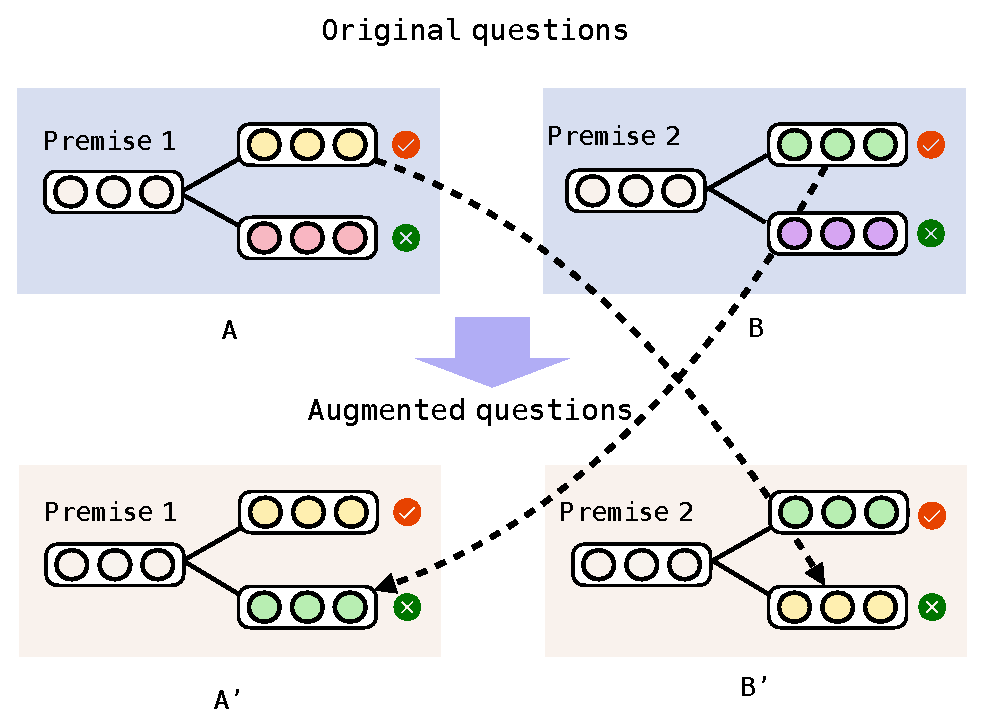
\includegraphics[width=\columnwidth]{figure/cross.eps}
\caption{The Crossover Operation: the true choice of both questions
are used to replace the false choices of these questions to create
two new proxy questions.}
\label{fig:cross}
\end{figure}

Compared to all other operations in classes 1 and 2, the crossover provides a proxy question that is most different from the original one but easier from a human perspective. This is because the two choices may be quite unrelated. If the model does not handle it correctly, it may be more indicative of a short circuit. As a result, the crossover is potentially a better short circuit test than others.

Another advantage of the crossover operation is that we can generate multiple false choices for an original question at a low cost, allowing us to test each original question more thoroughly. In contrast, most other operations cannot produce an adequate number of different variants of the original choice.

In summary, the proposed black-box choice operator provides a more generalizable and model-independent method for detecting short circuits in MCQ models. By applying various operations to create proxy questions, we can assess the model's performance and robustness more accurately, contributing to the development of better and more reliable models in the future.

\subsection{Improving Model Robustness by Data Augmentation}

If a model is shown to short-circuit by the proxy tests, its performance may decline, especially when applied to out-of-domain test data. To make models more robust, one natural thought is to generate more data to encourage models to focus on the relation between the premise and choices. While the operations used to generate proxy tests can also be utilized for data augmentation, not all of them are scalable or able to generate enough data for training.

The two operations that can generate a substantial amount of data are crossover and mutation. These operations can be applied to the training data to enhance the model's robustness.

\subsubsection*{Crossover for Data Augmentation}

Crossover is a good option for data augmentation because the two choices were originally true answers in their respective questions and presumably carry spurious features if the model was short-circuiting. By incorporating crossover into the training data, the model is forced to consider the premise in order to determine which choice is better.

\subsubsection*{Mutation for Data Augmentation}

Mutation has two flavors: (1) swap the words only in the true choice; (2) swap the words both in the true and the false choice. Compared to crossover, mutation has the potential to be more effective at improving model robustness. It not only forces the model to look into the premise due to its two very similar choices (same set of tokens), but also makes the model more sensitive to fine differences in word orders and enhances the model's prior grammatical knowledge.

\subsubsection*{Differentiating between Proxy Test and Data Augmentation}

It is essential to differentiate between the use of crossover and mutation operations in proxy tests and data augmentation. In proxy tests, these operations are used to modify the test data to assess the model's short-circuiting behavior. In contrast, when applied for data augmentation, the same operations work on the training data to enhance the model's robustness and generalization capabilities.

In conclusion, data augmentation through crossover and mutation operations can contribute to improving model robustness by encouraging models to focus on the relationship between the premise and choices. By incorporating these operations into the training data, models are forced to consider the premise and become more sensitive to the fine differences in word orders, leading to better performance and reliability in real-world applications.



\section{Experiment}
In this section, we experiment on different NLG tasks. We first present the experimental setup on different tasks. Then, we show the quantitative and qualitative results together with comprehensive analysis and ablation studies.

\subsection{Implementation Details}
We evaluate the newly proposed ICL strategy on five commonly-researched natural language generation tasks: reading comprehension, dialogue summarization, style transfer, question generation and news summarization. Details on the task description, the strong baseline, corresponding  dataset, evaluation metrics and key hyper-parameters for each task are presented as follows.

\begin{table*}[th]
	\scriptsize
	\centering
	\begin{tabular}{lp{1.1cm}rrrcccc}
		\hline
		Task & Dataset & \#Train & \#Val & \#Test & Input & Output & Avg & Std\\
		\hline
		Reading Comprehension & DREAM & 6,116 & 2,040 & 2,041 & ``Q:''+ question + dialogue & answer & 5.59 & 2.61\\
		Dialogue Summarization & SAMSum & 14,732 & 818 & 819 & dialogue & summary  & 24.99 & 13.06\\
		Style Transfer & Shakespeare & 36,790 & 2,436 & 2,924 & original/modern  & modern/original  & 11.63 & 8.19 \\
		Question Generation & SQuAD1.1 & 75,722 & 10,570 & 11,877 & passage + [SEP] + answer & question & 13.09 & 4.27 \\
		News Summarization & CNNDM & 287,227& 13,368& 11,490 & document & summary & 70.97 & 29.59\\ 
		\hline
	\end{tabular}
	\caption{A summary of tasks and datasets. \#Train, \#Val and \#Test refers to the number of samples in the corresponding dataset. Avg and Std are the statistics for the number of output tokens. ``+'' refers to the concatenation operation.}
	\label{tab:taskdata}
\end{table*}

\textbf{Reading comprehension} is the task that answering questions about a piece of text. We use the DREAM dataset~\cite{sun2019dream} where questions are about corresponding dialogues and the answer is a complete sentence in natural language. We neglect the negative choices in the original dataset and formulate it as a NLG task. We adopt the pre-trained language model BART~\cite{lewis2020bart} as the baseline, where the input is a concatenation of a question and the corresponding dialogue made up of speakers and utterances. 
We experiment with  transformers\footnote{\url{https://github.com/huggingface/transformers}} based on the publically available ``facebook/bart-large'' checkpoint \footnote{\url{https://huggingface.co/facebook/bart-large}}.
%The preceding BART model is also adopted as the baseline, whereas the input is a concatenation of question and a dialogue.
The generated answers are evaluated by BLEU scores\footnote{The BLEU-1/2/3/4 scores are computed according the Google's implementation(\url{https://github.com/tensorflow/nmt/blob/master/nmt/scripts/bleu.py}).}~\cite{papineni2002bleu} widely used for QA systems, together with Meteor and Rouge-L F1 as mentioned above. The parameters are also the same as dialogue summarization, except that the early-stop is activated if there is no improvement on the perplexity of the validation set. 


\textbf{Dialogue summarization} is to generate a concise summary covering the salient information in the input dialogue. The preceding model BART has shown to be a strong baseline for this task, where only the dialogue is concatenated into a single sequence as the input. We experiment with  %transformers\footnote{\url{https://github.com/huggingface/transformers}} based on the publically available ``facebook/bart-large'' checkpoint \footnote{\url{https://huggingface.co/facebook/bart-large}} and 
SAMSum dataset\footnote{\url{https://arxiv.org/src/1911.12237v2/anc/corpus.7z}}~\cite{gliwa2019samsum} for daily-chat dialogues. 
The generated summaries are evaluated by comparing with the reference through evaluation metrics, including Rouge-1/2/L F1 scores\footnote{\url{https://github.com/pltrdy/files2rouge}}~\cite{lin2004rouge}, Meteor~\cite{banerjee2005meteor} and BertScore F1\footnote{Both Meteor and BertScore are calculated by SummEval(\url{https://github.com/Yale-LILY/SummEval}), and the latter one is based on the default bert-base-uncased model.}. We evaluate the model on the validation set after each training epoch and the early-stop patience will be added 1 if there is no improvement according to the Rouge-2 F1 score. The training process terminates when the early-stop patience equals or is larger than 3.  During the inference, the minimum and maximum output length is set to 5 and 100 respectively, with no\_repeat\_ngram\_size=3, length\_penalty=1.0 and num\_beams=4.


% The answer is either a span of words in the original text or a complete sentence in natural language.
\textbf{Style transfer} preserves the semantic meaning of a given sentence while modifies it's style, such as positive to negative, formal to informal, etc.
We adopt the Shakespeare author imitation dataset~\cite{xu2012paraphrasing}, containing William Shakespeare's original plays and corresponding modernized versions. Krishna el al.~\shortcite{krishna2020reformulating} proposed to do unsupervised style transfer by training paraphrase models based on the GPT-2 language model~\cite{radford2019language}. We re-implemented their approach STRAT\footnote{\url{https://github.com/martiansideofthemoon/style-transfer-paraphrase}} and evaluated with the provided script. Evaluation metrics includes 
transfer accuracy(ACC), semantic similarity(SIM), Fluency(FL) and two aggregation metrics, i.e., geometric averaging(GM) and their newly introduced $J(\cdot)$ metric. The hyper-parameter $hp$ equaling 0.0, 0.6 or 0.9  in Table~\ref{tab:end2endst} is the sampling parameter for trades off between ACC and SIM in their approach. 
In the training stage, we evaluate the model after updating every 500 steps. The perplexity on the validation set is used to activate the early-stop which equals 3. The inference is done as default.
 
\textbf{Question generation}~\cite{zhou2017neural} aims at generating a question given an input document and its corresponding answer span. SQuAD 1.1~\cite{rajpurkar2016squad} is generally used for evaluation. We adopt the data split as in \cite{du2017learning} and fine-tune the pre-trained UniLM~\cite{dong2019unified} as the strong baseline according to their official implementation\footnote{\url{https://github.com/microsoft/unilm/tree/master/unilm-v1}}. Generated questions are evaluated by metrics including BLEU-1/2/3/4, Meteor and Rouge-L with the provided scripts. The model is evaluated every 1000 steps and the early-stop equaling 3 is associated with the perplexity on the validation set. Other parameters are unchanged following the official guideline.

\textbf{News summarization} differs from dialogue summarization where the input is a document instead of a dialogue. We adopt the same strong baseline BART and evaluation metrics as dialogue summarization. Experiments are done with CNNDM dataset~\cite{HermannKGEKSB15} consisting of news articles and multi-sentence summaries\footnote{\url{https://github.com/pytorch/fairseq/blob/main/examples/bart/README.summarization.md}}. The model is evaluated every 2000 steps and the early-stop equaling 3 is associated with the Rouge-2 on the validation set. During the inference, the minimum and maximum output length is set to 45 and 140 respectively, with no\_repeat\_ngram\_size=3, length\_penalty=2.0 and num\_beams=4.
%\footnote{Inference parameters are borrowed from \url{https://github.com/pytorch/fairseq/blob/main/examples/bart/summarize.py}}

The summary of each task is listed in Table~\ref{tab:taskdata}. For fair comparisons, we re-implemented baselines following the above instructions on our machine. On top of the above baselines, we further arm them with the ICL strategy according to the Algorithm~\ref{alg:picl}. The settings of newly introduce Start and Stride are specified and discussed in following sub-sections. All of our experiments are done on a single RTX 3090 or a single RTX 2080Ti with 24G and 11G GPU memory respectively.
%and the result are averaged over three runs.


 
\subsection{Automatic Evaluations on Different Tasks}
\label{sec:taskperformances}

We compare our approach with the vanilla models mentioned above and the approach from~\citet{liang-etal-2021-token-wise} as baselines.
The performances on different NLG tasks are shown in Table~\ref{tab:end2end}. 
These tasks not only focus on solving different problems, but also has various amount of training data as well
as reference output lengths as shown
Table~\ref{tab:taskdata}.
Besides, the basic model are also different, including BART, GPT-2 and UniLM. 
Our new training strategy achieves significantly improvements among different tasks on most evaluation metrics, which shows that our method not only works well, but also has strong generalization abilities.

We explain the some specific results as follows:

(1) Our training strategy boosts the performances of the original STRAT with different $hp$ in the style transfer task. GM and J are two comprehensive evaluation metrics, with our approach topping the ranks with significant improvements.

(2) TCL generally performs poorly on tasks
with more training data. For example, it failed on question generation without any improvements over the vanilla model under the same parameter setting, while ICL still 
logs gains. This is mainly due to two reasons.
First, because the nature of TCL is data augmentation which is more effective in low-resource settings,
when training data is abundant, it becomes less useful. 
Second, the way they calculate the loss as sub-sequence generation better suites paraphrasing tasks, such as machine translation tested in their paper, as the order of 
the corresponding tokens between input and output 
are almost the same. Learning such forward mapping can 
be regarded as a kind of ``easy-to-hard'' 
in these limited scenarios.
However, this doesn't hold true for other tasks, 
such as summarization and question generation. 
Therefore, we didn't further test it on CNNDM since
CNNDM has the large amount of training data among
the five.

(3) For news summarization, Rouge-1 scores (precision, recall) for the baseline and our method on CNNDM are (38.16, 52.72) and (40.84, 49.23) correspondingly. Our method made substantial improvements on the precision with a compromise on the recall. 
The meteor score based on the unigram precision and recall emphasizes more on the recall than the Rouge-1 F1. As a result, it drops while Rouge-1 F1 increases. Overall, our method still outperforms BART on this task, especially on F1 scores of Rouge-2 and Rouge-L.




\begin{table}[th]
	\small
	\centering
	\begin{subtable}{\linewidth}
		\scriptsize
		\centering
		\begin{tabular}{lcccccc}
			\hline
			{Method} & {B1} & {B2} & {B3} & {B4} & {Met} & {RL}\\
			\hline
			w/o CL &  32.03 & 16.01 & 8.77 & \textbf{4.80} & 19.84 & 38.89\\
			TCL & 32.53 & 16.25 & 8.52 &4.67 &19.88 & 39.65 \\
			ICL &  \underline{\textbf{33.99}} & \underline{\textbf{17.43}} & \underline{\textbf{9.18 }}& 4.64 & \textbf{20.60} & \textbf{40.78}\\

			\hline
		\end{tabular}
		\caption{Reading Comprehension}
		\label{tab:end2endrc}
	\end{subtable}
	\\[5pt]
	\begin{subtable}{\linewidth}
		\scriptsize
		\centering
		\begin{tabular}{lccccc}
			\hline
			{Method} & {R1} & {R2} & {RL} & {Met} & {BertS} \\
			\hline
			%BART & 52.60&27.00 &42.10 &- & - \\
			w/o CL & 51.88 & 27.30 & 42.77 & 24.75 & 71.38 \\
			TCL  & 52.33 & 27.80 & \textbf{43.91} & 24.59 & 71.77 \\
			ICL & \underline{\textbf{53.07}} & \underline{\textbf{28.23}} & {43.83} & \underline{\textbf{26.12}}& \underline{\textbf{72.17}} \\
			
			\hline
		\end{tabular}
		\caption{Dialogue Summarization}
		\label{tab:end2endds}
	\end{subtable}
	\\[5pt]
	\begin{subtable}{\linewidth}
		\scriptsize
		\centering
		\begin{tabular}{lcccccc}
			
			\hline
			{Method}&$hp$ &  {ACC} & {SIM} & {FL} & {GM} & {J}\\
			\hline
			%\multirow{3}{*}{STRAT}& 0.0 & 71.70 & \textbf{56.40} & 85.20 & 70.10 & 34.70 \\
			%& 0.6 & 75.70 & 53.70 & 82.70 & 69.50 & 33.50 \\
			%& 0.9 & 79.80 & 47.60 & 71.70 & 64.80 & 27.50 \\
			%\hline
			\multirow{3}{*}{w/o CL}& 0.0 & 70.49 & 55.70 & 85.98 & 69.63& 33.72 \\
			& 0.6 &75.31 & 53.46 & 82.56 & 69.27& 33.30\\
			& 0.9 & 78.76 & 47.38 & 74.42 &65.24 & 27.88\\
						\hline
			\multirow{3}{*}{TCL } & 0.0 & 70.31 & \textbf{55.95} &\textbf{87.24} &  70.01& 34.71 \\
			& 0.6 & 74.79 & 53.14 & 82.56 & 68.97 & 33.21 \\
			& 0.9 & 79.41 & 46.88 & 71.92 &64.45 & 26.92 \\
			\hline
			\multirow{3}{*}{ICL}& 0.0 & \underline{73.72} & 55.91 & 86.30 & \underline{\textbf{70.60}} &\underline{\textbf{35.81}}\\
			& 0.6 & 77.26 & \underline{53.80} & \underline{83.87} & \underline{70.38} & 34.64\\
			& 0.9 & \textbf{79.65} & 48.16 & 76.06 & 66.32 & 29.03\\

			\hline
		\end{tabular}
		\caption{Style Transfer.}
		\label{tab:end2endst}
	\end{subtable}
	\\[5pt]
	\begin{subtable}{\linewidth}
		\scriptsize
		\centering
		\begin{tabular}{lcccccc}
			\hline
			{Method} & {B1} & {B2} & {B3} & {B4} & {Met} & {RL}\\
			\hline
			w/o CL & \textbf{50.38} & 35.67 & 27.24 & 21.36 & 24.40 & 50.67 \\
			TCL &\textbf{50.38} & 35.67 & 27.24 & 21.36 & 24.40 & 50.67\\
			ICL &  50.18 & \textbf{35.72} & \textbf{27.36} & \textbf{21.54} & \textbf{24.57} & \underline{\textbf{51.09}} \\
			\hline
		\end{tabular}
		\caption{Question Generation}
		\label{tab:end2endqg}
	\end{subtable}
		\\[5pt]
	\begin{subtable}{\linewidth}
		\scriptsize
		\centering
		\begin{tabular}{lccccc}
			\hline
			{Method} & {R1} & {R2} & {RL} & {Met} & {BertS}\\
			\hline
			%BART &  \\
			w/o CL &  43.07 & 20.01 & 35.94 & \textbf{21.44} & 63.72 \\
			TCL & - & -&- &- &- \\
			ICL & \textbf{43.39} & \underline{\textbf{20.55}} & \underline{\textbf{36.63}} & 19.68 & \textbf{64.05}\\
			\hline
		\end{tabular}
		\caption{News Summarization}
		\label{tab:end2endns}
	\end{subtable}
	\caption{Performances on different NLG tasks. ICL represents the models trained with our ICL algorithm. TCL refers to the previous work from~\cite{liang-etal-2021-token-wise}. Scores underlined are statistically significantly better than both re-implemented baselines with $p<0.05$ according to t-test. }	
	\label{tab:end2end}
\end{table}


\subsection{Human Evaluations}

To further prove the improvement of ICL, we hired three proficient English speakers for human evaluation. 20 samples from the test set of each task are randomly selected, ignoring the ones with totally same generations among three models, including the vanilla model, TCL and ICL. The original input, reference output and three generations are shown to annotators together, while the order of three generations are unknown and different among samples. 3-point Likert Scale is adopted for scoring for each generation~\cite{gliwa2019samsum}, where [1, 3, 5] represent 
excellent, moderate and disappointing results 
respectively. The average scores and agreements 
among the annotators are shown in 
Table~\ref{tab:humaneval}.

The Fleiss Kappa on the first four tasks indicates the fair to moderate agreements. It shows the promising improvement of ICL over the vanilla model and TCL especially on DREAM, SAMSum, and SQuAD1.1, which is consistent with the conclusion based on automatic metrics.
Although the agreement on style transfer is fair, 
our annotators without Shakespeare background 
tend to give low scores to all outputs.
Therefore, the absolute improvement is 
only $0.04$ compared to both baselines.
%This mainly due to the indistinguishable styles between
%Shakespeare’s plays with are quite different from modern languages. 
Besides, the poor agreement on CNNDM reflects the 
diverse concerns of summarization from different 
annotators. Without more specific instructions, they 
tends to focus more on the content coverage instead 
of checking the detailed facts. This is also 
consistent with the higher Meteor scores of the 
vanilla model over ICL.

\begin{table}[th]
	\scriptsize
	\centering
	\begin{tabular}{l|ccc|c}
		\hline
		{Datasets} & {w/o CL} & {TCL} & {ICL} & {Agreement}  \\
		\hline
		DREAM  &3.07 & 2.50&3.20 &0.48 \\
		SAMSum &2.97 &3.57 &3.97 &0.40 \\
		Shakespeare &2.23 &2.23 & 2.27&0.32 \\
		SQuAD1.1 &3.43 & 3.43 &3.77 &0.35 \\
		CNNDM & 3.45 &- &3.40 &0.11 \\
	%	\hline
	%	overall & & & &\\
		\hline
	\end{tabular}
	\caption{Human evaluations. The agreement is calculated by Fleiss Kappa.}
	\label{tab:humaneval}
\end{table}




%Following Liu et al.\shortcite{liu2021competence}'s work, we asked annotators to comparing the performance between our generated results and baselines by choosing from ``Better, Tie, Worse''. 
%The counts for each choice are shown in Table~\cite{}, where the Fleiss Kappa among annotators is ??.

%Analysis





%\subsection{Analysis on Variable Generation Lengths}

%Teacher forcing, which predicts each token given the reference summary tokens during training and given the previous generated tokens during inference, leads to the exposure bias problem for NLG tasks.
%Since ICL starts the training process by predicting the last few tokens of outputs and gradually calculates the loss based on more tokens when the model is stronger, we hypothesis that it can alleviate the exposure bias for training Seq2Seq models to some extent.
%As stated in~\cite{pang2020text}, the output quality tends to degrade as the output length increase with the exposure bias.
%So, we divided the test set of each task according to the length of the generated output into 4 buckets and randomly picked 20 samples in each buckets for both the corresponding baselines and our approach. Each generation is annotated by 5 point Likert Scale, where 1 is the worst and 5 is the best. 

%The trends of performances on variable generation lengths are in Figure~\ref{}.



\subsection{Different Decoder Models}
Zheng et al. used relative complex variant of LSTM as the simple RE tagging
decoder. Evaluate the effectiveness of different alternatives, 
we compare Zheng's LSTM cell with two popular
RNN cells, namely normal LSTM and GRU on the basic RE tagging task.
To enable comparison with Zheng's results, we use order-first algorithm to
construct triples. \tabref{tab:decode} shows the results.

\begin{table}[th!]
  \begin{center}
  \small
  \caption{Results from Different Decoders}
  \label{tab:decode}
    \begin{tabular}{c|ccc}
      \hline
      \bf Models & \bf Prec. & \bf Rec. & \bf F1 \\
      \hline
      Zheng-LSTM  & \textbf{.615} & .414 & .495 \\
      LSTM   & .592 & .444 & \textbf{.507} \\
      GRU    & .579 & .438 & .499 \\
      \hline
    \end{tabular}
  \end{center}
\end{table}

Vanilla LSTM beats the rest by narrow margin in F1. 
We can conclude that Zheng's complex LSTM is not any better than the
basic LSTM, therefore in all other experiments, we adopt the vanilla
LSTM as our decoder.
%no much difference in F1 value between 4 LSTM cells. This conclusion is
%consistent with many work by others. However, the ability to balance precision
%and recall is really diffenrent. The difference between precision and recall
%values is beyond $0.20$, while this difference of any one of other 3 LSTM cell
%is limited in $0.15$. The precision value of Zheng is the highest and the recall
%is the lowest. Therefore,  we choose Pure-LSTM as our decoder in later experiments.


\subsection{Different Construction Algorithm}
In this experiment, we compare three different triple construction algorithms
in \tabref{tab:cons1}. $e_1$-first algorithm has a clear advantage
than $e_2$-first, which is in turn better than the default order-first.
This can be explained if we look at the accuracy of $e_1$ and $e_2$ in
the RE-tagging results in \tabref{tab:cons2}.
\begin{table}[th!]
  \small
  \begin{center}
  \caption{Different Construction Algorithms on Triple Accuracy}
  \label{tab:cons1}
    \begin{tabular}{c|ccc}
      \hline
      \bf Models & \bf Prec. & \bf Rec. & \bf F1 \\
      \hline
      $e_1$-first   &  \textbf{.631} & \textbf{.480} & \textbf{.545}  \\
      $e_2$-first   &  .605 & .450 & .516  \\
      Order-first  &  .592 & .444 & .507  \\
      \hline
    \end{tabular}
  \end{center}
\end{table}

\KZ{Add another algorithm that gives the nearest pairs.}
From \tabref{tab:cons2}, the accuracy for tagging $e_1$ is higher than
$e_2$ consistently. \KZ{Why is that?} As a result, the $e_1$-centric 
triple construction algorithm gives better overall accuracy than if we
use $e_2$ as the dominating entity. Order-first algorithm is worst because
it imposes a strict order of selecting entity pairs, which is more brittle
than other two algorithms. In the rest of this section, we will
use $e_1$-first as our triple construction algorithm.

\begin{table}[th!]
  \small
  \begin{center}
  \caption{RE Tagging Accuracy on the Entities}
  \label{tab:cons2}
    \begin{tabular}{ccc|ccc}
      \hline
       \multicolumn{3}{c|}{$e_1$} & \multicolumn{3}{c}{$e_2$} \\
      \hline
      	 Prec. & Rec. & F1 & Prec. & Rec. & F1 \\
      \hline
%        .650 & .606 & .627 & .616 & .603 & .609 \\
        .660 & .603 & .630 & .622 & .600 & .610 \\
%        .653 & .594 & .621 & .620 & .601 & {\bf .610} \\
      \hline
    \end{tabular}
  \end{center}
\end{table}



%As we can see from table 3, Order-First is worst, and Ele2-First is a little better
%than Order-First. Ele1-First is the best algorithm which achieve near $4$
%percent points than Order-First. The reason can be found in tabel 4 which show
%the preformance on signle element and element pair.
%
%The metrics on $e_1$ and elment2 is very near between these 3 experiments.
%Because the only different between these 3 experiments is the construction algorithm
%which do not take part in the training process. The ability to predict correct tag
%sequence should be near each other. The prediction of signle element has nothing
%to do with construction algorithm. By comparing the performance of $e_1$ and
%$e_2$, we can find the ability to predict correct $e_1$ is pretty high
%than $e_2$. The recall value of $e_1$ and $e_2$ is all most the same.
%But the precision values have a big difference. This means the model has predict
%more wrong $e_2$ than $e_1$. In other word, there is more correct $e_1$
%than $e_2$. Therefore, it is better to choose $e_1$ as the dominating
%entity rather than $e_2$. This is the reason why Ele1-Frist outperforms
%Ele2-First a lot. Order-First treats $e_1$ and $e_2$ in equal position
%which means this algorithm depends on the accuracy of both $e_1$ and
%$e_2$. In other words, the performance of Order-First is limited by the worse
%one of the two elements. This is the reason why Order-First is a little worse
%than Ele2-Frist.

\subsection{End-to-end RE Results}
%We have proved Pure-LSTM is more suitable for the decoder of EndRE module in 4
%kinds of LSTM cells. And Ele1-First algorithm is the best one to construct
%triple from relation tag sequence. We test the performance of our full
%multi-task model based on Pure-LSTM and Ele1-Frist algorithm. 
\tabref{tab:e2e} shows the accuracy of end-to-end relation triple extraction from
all baseline methods as well as our methods. Because our method enhances
Zheng's LSTM-LSTM-Bias (LLB) model, we name our method LLB+, which means
LLB plus RTD.

\begin{table}[th!]
  \small
  \begin{center}
    \begin{tabular}{cccc}
      \hline
      \bf Models & \bf Prec. & \bf Rec. & \bf F1 \\
      \hline
      FCM & .553 & .154 & .240 \\
      DS+logistic & .258 & .393 & .311 \\
      LINE & .335 & .329 & .332 \\
      \hline
      MultiR & .338 & .327 & .333 \\
      DS-Joint & .574 & .256 & .354 \\
      CoType & .423 & .511 & .463 \\
      \hline
      LSTM-CRF & \textbf{.693} & .310 & .428 \\
      LSTM-LSTM & .682 & .320 & .436 \\
      LSTM-LSTM-Bias & .615 & .414 & .495 \\
      \hline
      LLB+ & .623 & \textbf{.517} & \textbf{.565} \\
%      LLB+ (-NER) & .618 & .513 & .561 \\
      LLB+ (-RTD) & .618 & .498 & .552 \\
%      LLB+ (-NER-RTD) & .631 & .480 & .545 \\
      \hline
    \end{tabular}
  \end{center}
  \caption{End-to-end RE Results}
  \label{tab:e2e}
\end{table}

\begin{table*}[th!]
  \small
  \begin{center}
  \caption{Accuracy of Entity Tagging}
  \label{tab:entity}
    \begin{tabular}{c|ccc|ccc}
      \hline
      Entity & \multicolumn{3}{|c|}{E1} & \multicolumn{3}{|c}{E2} \\
      \hline
      	& Prec. & Rec. & F1 & Prec. & Rec. & F1 \\
      \hline
      LSTM-CRF & .596 & .325 & .420 & .605 & .325 & .423 \\
      LSTM-LSTM & .593 & .342 & .434 & .619 & .334 & .434 \\
      LSTM-LSTM-Bias & .590 & .479 & .529 & .597 & .451 & .514 \\
      \hline
      LLB+  & .628 & .657 & .642 & .594 & .647 & .619 \\
%      LLB+ (-NER) & .620 & .649 & .634 & .589 & .645 & .615 \\
      LLB+ (-RTD) & .623 & .661 & .641 & .592 & .647 & .618 \\
%      LLB+ (-NER-RTD) & .650 & .606 & .627 & .616 & .603 & .609 \\
      \hline
    \end{tabular}
  \end{center}
\end{table*}

Compared to the state-of-art model LSTM-LSTM-Bias, our method LLB+
logged 7\% substantial improvement on F1. This gain is primarily due to 
the advantage in recall, which is more than 10\%. 
%The precision values between LSTM-LSTM-Bias and MT-EndRE is not different
%too much, but MT-EndRE improve the recall value very much which achieves more
%than $10$ percent points gain. 
By looking at the accuracying of tagging $e_1$ and $e_2$ in \tabref{tab:entity}, 
we see that the recall of both $e_1$ and $e_2$ improve dramatically over 
LSTM-LSTM-Bias, while the precision remains relatively unchanged. 
This means our multi-task model predicts more entity pairs correctly
without lowering the precision.
%Therefore, our model can achieve remarkable gain in recall of relation triple.
%Finally, MT-EndRE can beat the state-of-the-art model a lot. Also our multi-task
%model is much better than all the pipeline and joint approches.

Further, to show the effect of the two auxiliary tasks in our model, we conduct
the ablation tests (shown in lowest section of \tabref{tab:e2e}). 
We find that the auxiliary task RTD is useful in boosting the basic RE model. 
%while RTD task provides more boost than NER.  
%LLB+(-NER-RTD) is the model without NER and RTD module 
%which is just the RE tagging module by itself. By comparing with full multi-task model
%MT-EndRE, without NER module the F1 value of triple will drop a little while
%without RTD module the F1 value will drop more. If getting rid of both NER and
%RTD, the performance will drop a lot. This means RTD module can provide more
%help to the EndRE by comparision with NER. There may be two reasons which cause
%RTD is more helpful than NER. 
This is because 
%i) NER is a relatively easy task, and previous research has shown
%accuracy above 0.92, so the basic RE tagging module itself can handle it
%rather well; ii) 
RC is a harder task but its relative, RTD, is able to  
provide global information of whole sentence which
complement the information obtained by the RE tagging alone. 
\KZ{Say a little more here?}

\subsection{Case Study}
To illustrate the effectiveness of our proposal, we present two cases
from the test set. The first sentence is used to show the effectiveness of our
joint model LLB+ by comparing with LLB. \{India, Contains, Bihar\} is the gold
triple. Both LLB+ and LLB mistake the number ``351'' as $e_2$ because
of the misleading context ``in''. Based on the tag of ``351'', LLB treat
``Bihar'' as the $e_2$ which is wrong. However, the LLB+ model 
predicts ``Bihar'' as $e_2$ which seems to conflict with the existing $e_2$ ``351''.
``India'' is predicted as $e_1$ correctly for two models. Eventually, 
LLB+ succeeds in constructing the correct triple. 
This is because LLB heavily relies on the local information (nearby entities) 
while LLB+ has a more global view.

The second sentence illustrates the difference between the triple construction
algorithms. In this case, all of the construction algorithms operates on the
same RE tag sequence. $e_x$-first re-constructs the correct triple \{Iowa,
Contains, Waverly\} while order-first does not. Because this tag sequence contain
several redundant $e_2$, the correct $e_2$ is the nearest to $e_1$ ``Iowa''.
However, order-first algorithm re-constructs the wrong triples \{Iowa,
Contains, Wartburg College\}. As for $e_2$-First, it only
predicts the two correct entities, it can only re-construct one triple which is
the correct one. \KZ{Find another example with the same tag sequence.}

\begin{table*}[th!]
  \small
  \begin{center}
  \caption{Two Examples in Case Study}
  \label{tab:case}
    \begin{tabular}{lp{12cm}}
      \hline
      Gold Standard 1& the death toll stood at 351 in Bihar[Contains-2-S] state , which is home to this village and many others sitting on some of the most vulnerable floodplains in India[Contains-1-S] . \\
      LLB+ & the death toll stood at 351[Contains-2-S] in Bihar[Contains-2-S] state , ... the most vulnerable floodplains in India[Contains-1-S] . \\
      LLB & the death toll stood at 351[Contains-2-S] in Bihar[Country-1-S] state , ...  the most vulnerable floodplains in India[Contains-1-S] . \\
      \hline
      Gold Standard 2 & Jean-Luc Portal , 51 , a wine consultant in Somers[Contains-2-S] who grew up in the tiny village of Alzonne[Contains-2-S] in southern France[Contains-1-S] , said he became obsessed with the game when he was 6 . \\
      LLB ($e_1$-First) & \{ France, Contains, Alzonne \} \\
      LLB ($e_2$-First) & \{ France, Contains, Somers \} \\
      LLB (Order-First) & \{ France, Contains, Somers \} \\
      \hline
    \end{tabular}
  \end{center}
\end{table*}






\section{Related Work}
%Ruolan should write this part.
Early work on rewriting often considers the problem as a 
standard text generation task,
using pointer networks 
or sequence-to-sequence models %\citep{elgohary-etal-2019-unpack,quan-etal-2019-gecor} 
with a copy mechanism 
\citep{su-etal-2019-improving,elgohary-etal-2019-unpack,quan-etal-2019-gecor}
to fetch the relevant information in the context \citep{gu-etal-2016-incorporating}.
Later, pre-trained model like T5 \citep{2020t5} are fine-tuned with conversational 
query reformulation dataset to generate the rewritten utterance directly. \citet{DBLP:journals/corr/abs-2204-03958} uses Picker which identifies the omitted tokens to optimize T5. We the results in their paper, 
therefore, we did not compare with it in the experiments. In general, these generative approaches ignore the characteristic of IUR problem: rewritten utterances often share the same syntactic structure as the original incomplete utterances.

Given that coreference is a major 
source of incompleteness of an utterance,
another common thought is to utilize a 
coreference resolution or corresponding 
feartures. 
\citet{tseng-etal-2021-cread} 
proposed a model which jointly learns coreference resolution
and query rewrite 
with the GPT-2 architecture \citep{Radford2019LanguageMA}.
By first predicting coreference links
between the query and context,
the performance of rewriting has improved 
while the incompleteness is induced
by coreference.
However, this does not work for utterances
with ellipisis. Besides, the performance of 
the rewriting
 model is limited by
the coreference resolution model.

Recently, some of the work on 
incomplete utterance rewriting 
focuses on the ``actions'' we
take to change the original
incomplete utterance
into a self-contained
utterance (target utterance).
\citet{hao-etal-2021-rast} 
solves this problem  
%imcomplete utterance rewriting
with a sequence-tagging model.
For each word in the input utterance, 
the model will predict whether to
delete it or not, meanwhile, the
span of words which need to be inserted before
the current word will 
be chosen from the context.
\citet{liu-etal-2020-incomplete} 
formulated the problem as 
a syntactic segmentation task
by predicting 
segmentation
operations for 
the rewritten utterance.
\citet{DBLP:conf/icassp/ZhangLWCX22} extracts the coreference and omission relationship directly from the self-attention weight matrix of the transformer instead of word embeddings. Compared with these methods, our framework separates the two phases more thoroughly of predicting the rewriting position and filling in the blanks, and meanwhile, reduces the difficulty of the two phases with the divide and conquer method.
%directly extracting the coreference and omission relationship from the self-attention weight matrix of the transformer instead of word embeddings.
%\textcolor{blue}{Ruolan: could zitong please
%add 1 or 2 utterances to explain our advantage over
%sequence tagging and syntactic 
%segmentation approach?}
%Compared with these methods, our framework more thoroughly separates the two steps of predicting the rewriting position and filling in the rewriting content, and reduces the difficulty of the two steps with the divide and conquer method.

\section{Conclusion}
We implement a novel sequence-based dependency parsing
framework which takes advantage of high order features 
in parsing history. 
%We can also adapt beam search to this framework so as to
%relax the strictly greedy nature. Vine pruning\cite{rush2012vine} could
%be incorporated to speed up the parsing.
More importantly, we discovered that the parsing accuracy is very sensitive to
the quality of parsing sequence. Future work can be focused on
developing better sequence predictors that outperform Malt action classifier.
Furthermore, we use two sets of features for sequence predictor and
head mapper right now. A unified set of features between these two components
are worth exploring.
%Besides, better sequence predicting method and unified feature
%representation of two components are worth exploring.
%
%Though we currently get a not bad result,
%the sequence predictor still needs more exploration.
%According to our experiment, slightly changes
%on the sequence can lead to a fatal decline on accuracy. Ensuring the match degree of training sequence and testing
%sequence demands a high quality of sequence predictor.
%
%Further, the features in our current implementation are not expanded and well tuned yet  and we are free to define high order features to make use of parsing history. Our framework is flexible to merge other technics to enhance the performance. Introducing beam could make up for our greedy decoder and improve our accuracy. Vine pruning\cite{rush2012vine} could speed up parsing process. Besides, better sequence predicting method and unified feature representation of two components are worth exploring.


\section*{Acknowledgement}
This research was supported by the SJTU-CMBCC Joint Research Scheme, 
SJTU Medicine-Engineering Cross-disciplinary Research Scheme, and NSFC
grant 91646205.

\bibliographystyle{acl_natbib}
\bibliography{emnlp2020}

\end{document}
